%!TEX root = ../dissertation.tex
\chapter{Introduction}
\label{introduction}
Since 2012 \cite{krizhevsky2012imagenet}, the advent of deep learning has enabled researchers to study classical problems in computer vision such as object detection, semantic segmentation and instance segmentation, and achieve high performances in challenging datasets. These problems have lately been tackled using Convolutional Neural Networks (CNNs) \cite{DBLP:journals/corr/LongSD14}\cite{zhao2017pspnet}\cite{he_mask_2017} and insights into the information flow within such networks \cite{DBLP:journals/corr/HeZRS15}\cite{DBLP:journals/corr/HuangLW16a}, bearing in mind that CNNs are particularly well suited to process spatial and hierarchical information. 

On the other hand, Recurrent Neural Network (RNNs) models have been used previously to model and predict time sequences, these type of models have presented an state-of-the-art performance on different temporal-dependent applications, such as Speech Recognition \cite{DBLP:journals/corr/abs-1303-5778}, Handwriting recognition \cite{DBLP:journals/corr/Graves13}, text analysis and other specialized applications, such as protein reconstruction and nucleotide prediction \cite{doi:10.1093/bioinformatics/btw678}, and more recently on more advanced tasks such as Answering Open Domain Questions from large scale text corpus such as Wikipedia \cite{chen2017reading}. Moreover, several RNN models have been proposed, such as Long Short Term Memory (LSTM) \cite{Hochreiter:1997:LSM:1246443.1246450} units, Gated Recurrent Units (GRU) \cite{DBLP:journals/corr/ChoMGBSB14} and Simple Recurrent Units (SRU) \cite{DBLP:journals/corr/abs-1709-02755}, which presents the best time performance with respect to the previous models. However, all the aforementioned models are based on a set of state equations that relate both present input information at time $t$ with information from previous time steps $0 \cdots t-1$, allowing to model and generalize time dependent information, while removing unnecessary features that do not contribute to the generalization process.

Until now, most applications that blend language and vision are focused on Image Captioning \cite{DBLP:journals/corr/JohnsonKL15} \cite{DBLP:journals/corr/MaoHTCYM15} \cite{hendricks_deep_2015} \cite{gan_semantic_2016} \cite{johnson_densecap:_2016} \cite{yang_review_2016}, Visual Question Answering (VQA)  \cite{DBLP:journals/corr/ZhuGBF15} \cite{agrawal_vqa:_2015} \cite {goyal_making_2016} \cite{johnson_inferring_2017} \cite{teney_graph-structured_2016} and Image Retrieval based on Natural Language expressions \cite{hu_natural_2015} \cite{guadarrama_understanding_2016}. Most of the models proposed to handle these tasks are based on models that combine both visual and language modules (In the form of CNNs and RNNs), and while most modalities (Such as in VQA and Image Retrieval) receive both image and text as input to their models, they are not focused on producing a visual output such a segmentation or a detection target of the objects referred on the textual inputs.

Furthermore, due to the limited availability of datasets that combine both textual inputs and segmentation masks, most of the current available multimodal databases describe only an image and its object detection bounding boxes, alongside their corresponding natural language features, such as scene and attribute graphs and region descriptions, such as Visual Genome \cite{krishna_visual_2016}, one of the largest datasets in terms of visual and language relationships. However, this dataset is constrained to generate detection outputs, instead of segmentation masks.

To address this limitation, and acknowledging segmentation as a problem of high level, we propose to perform natural language-based object segmentation; this problem can be summarized as it follows: Given an image and a complex natural language query that contains references to a given set of object/s present on the image, produce a segmentation mask of the object/s referred. As it can be seen on Figure~\ref{Fig:Intro_Descr}, this problem differs from classic semantic segmentation by defining only two categories (Background/Belongs to the query), instead of $N$ object categories. For instance, an input image (\subref{subfig:original_img}) can have many output masks, depending on the input phrase

\begin{figure}
	\centering
    \begin{subfigure}[b]{0.25\columnwidth}
            \centering
            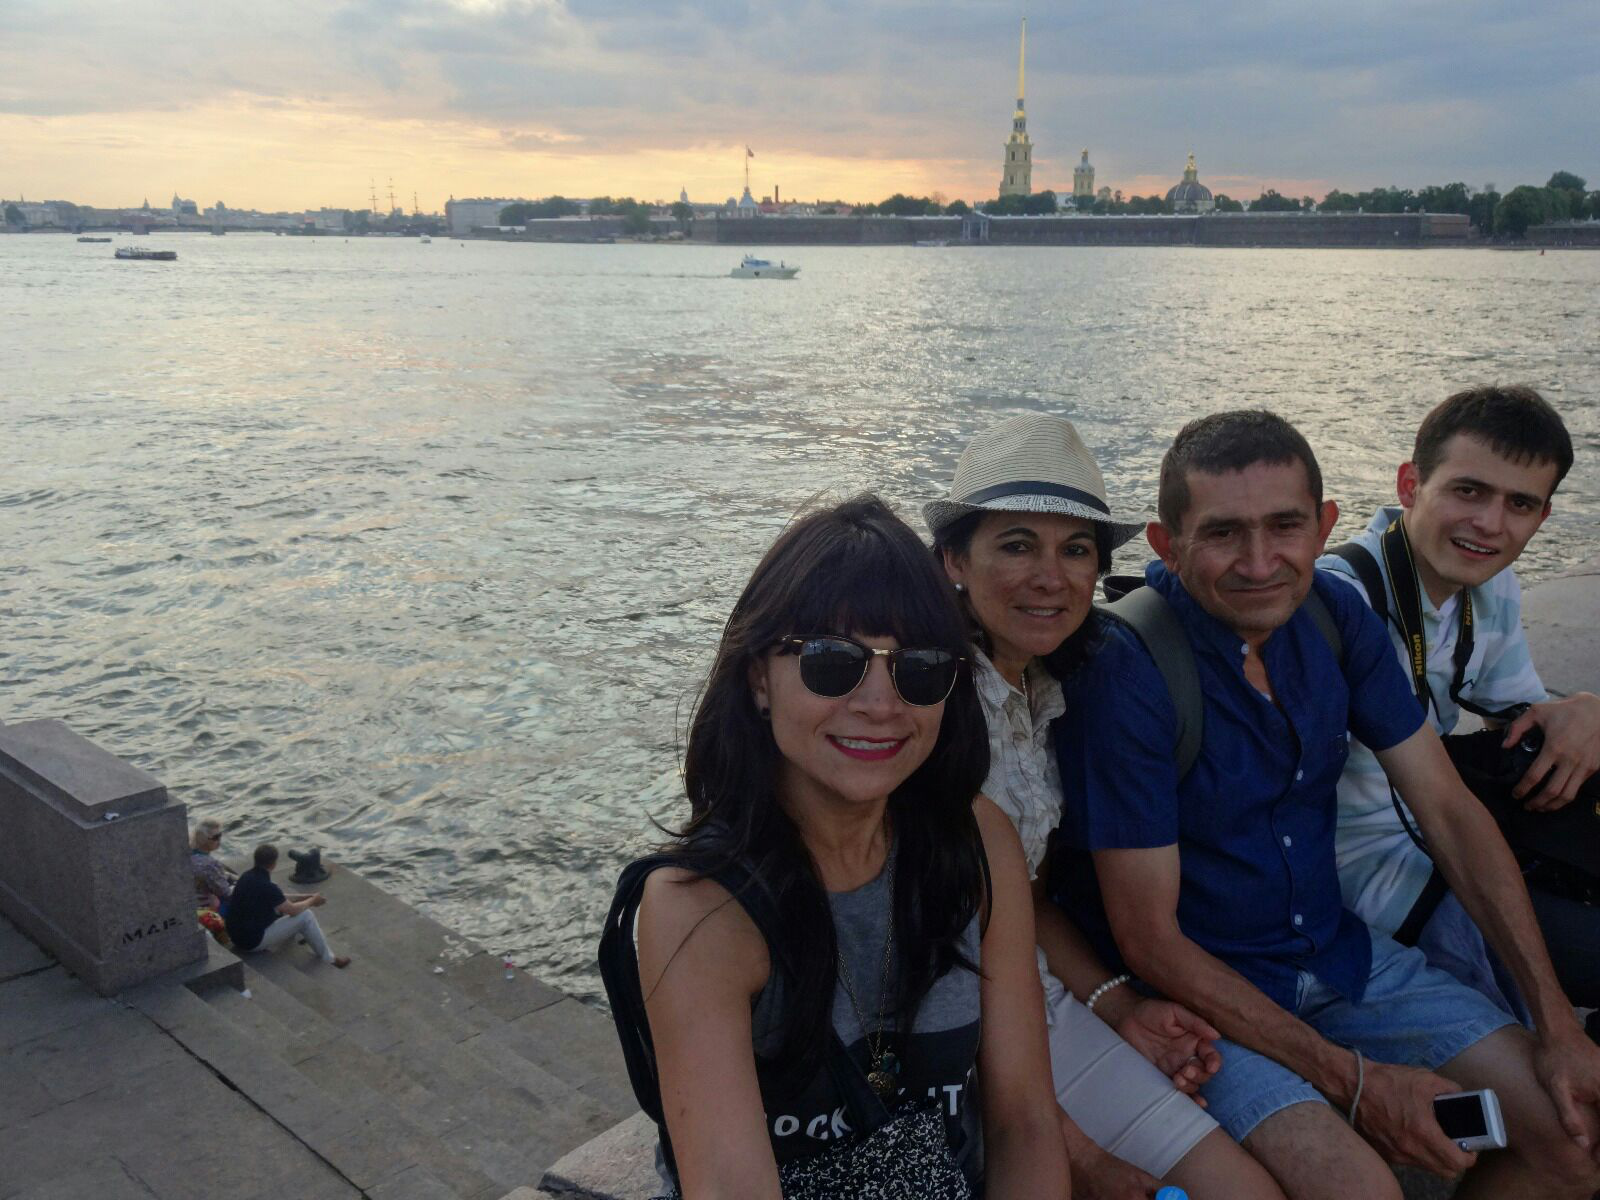
\includegraphics[width=\textwidth]{./figures/sample_image.png}
    \subcaption{Original Image}
    \label{subfig:original_img}
    \end{subfigure}
    \begin{subfigure}[b]{0.25\columnwidth}
            \centering
            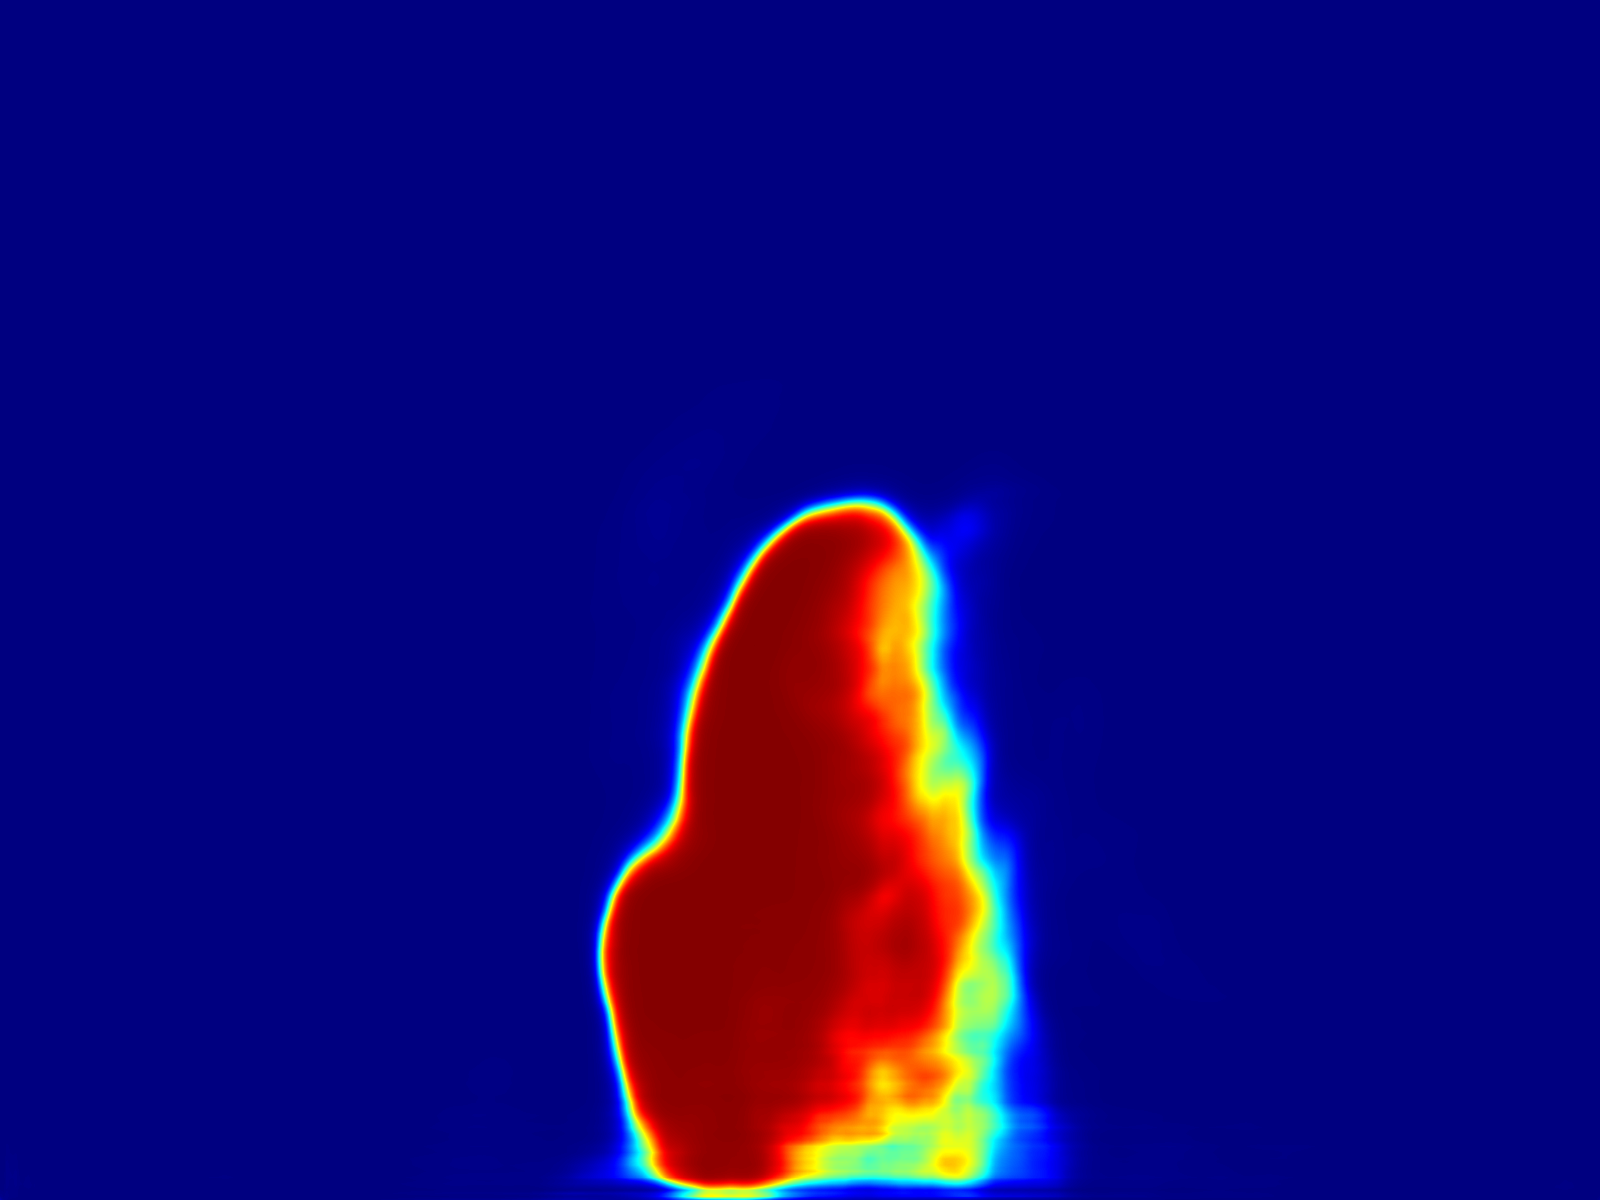
\includegraphics[width=\textwidth]{./figures/Mask_1.png}
    \subcaption{\textit{Woman on the left}}
    \label{subfig:woman_left}
    \end{subfigure}
     \begin{subfigure}[b]{0.25\columnwidth}
            \centering
            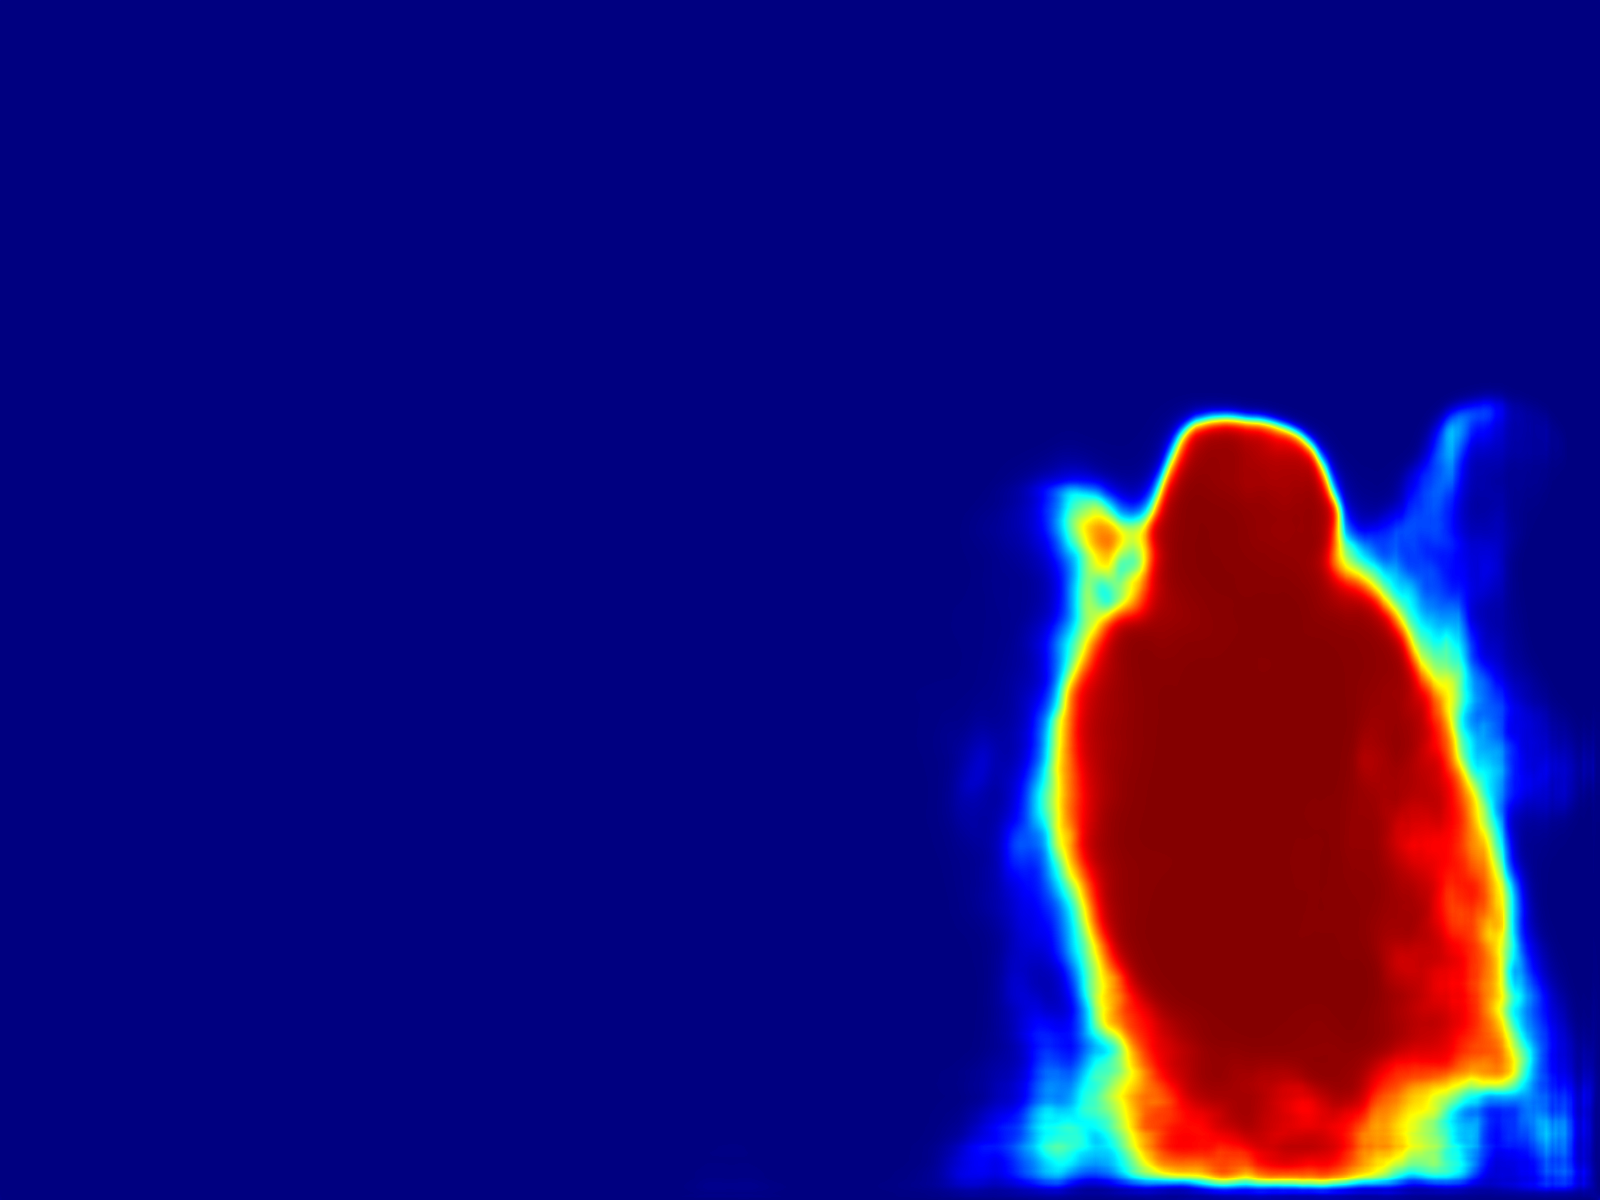
\includegraphics[width=\textwidth]{./figures/Mask_2.png}
    \subcaption{\textit{Man on blue}}
    \label{subfig:man_blue}
    \end{subfigure}
    %\subfloat[Original image.]{{\includegraphics[width=0.25\columnwidth]{./figures/first-fig-1.png} }}%
    %\quad
    %\subfloat[Heatmap based on query \textit{guy}.]{{\includegraphics[width=0.25\columnwidth]{./figures/first-fig-3.png} }}%
    %\quad
    %\subfloat[Heatmap based on query \textit{girl}.]{{\includegraphics[width=0.25\columnwidth]{./figures/girl.png} }}%
    \caption{\label{fig:query} Example of \textit{segmentation based on a natural language expression}. A single mask is the output, in which the only two labels represent \textit{member of query} and \textit{background}. Outputs are provided as heatmaps (\subref{subfig:woman_left}) and (\subref{subfig:man_blue})}
    \label{Fig:Intro_Descr}
\end{figure}

Besides, the model must have the ability to reason about the main object referred on the expression, as the number of possible expressions in the worst case that refer to same object is in the order of the length of all the combinations of words of a language vocabulary that contain a given object, whereas on Segmantic Segmentation a model must reason only about a constrained number of objects.

The applications of this problem are very varied, from robotics applications such as object retrieval based on natural language, such as in \cite{guadarrama_understanding_2016}, to image retrieval based on natural language descriptions \cite{schuster2015generating}; by providing a better scene and object understanding it is possible not only to retrieve images that contain an specific object, but also it is possible to retrieve the object itself. Finally, given multiple poses of the same object retrieved via a referring expression, it should be possible to reconstruct the object in 3D.

This problem aims to leverage a connection between all the main tasks on Computer Vision, as given by Malik's 3-R's of Computer Vision \cite{malik2016three}, and also with language recognition tasks. It is expected that the model should be able to \emph{Reorganize} an image information by focusing on certain objects or attributes of an image, \textit{i.e.,} Identify the main objects on the scene. Then it should be able to \emph{Recognize} the objects based on the language concept immersed on the referral expressions. Finally, from different view points and images that refer to the same object using the same referral expression, it should be possible to \emph{Reconstruct} the object.
